\documentclass[12pt]{article}
	\usepackage{amsmath}
	\usepackage{amssymb}
	\usepackage{fancyhdr}
	\usepackage{float}
	\usepackage{graphicx}
	\usepackage{cite}
	\usepackage{mathtools}

	\oddsidemargin0cm
	\topmargin-2cm     %I recommend adding these three lines to increase the 
	\textwidth16.5cm   %amount of usable space on the page (and save trees)
	\textheight23.5cm  

\newcommand{\myname}{Evan Palmer, Titouan Rigoudy}
\newcommand{\myandrew}{esp@andrew, trigoudy@andrew}
\newcommand{\myhwnum}{1}
\newcommand{\problemnum}{1}
\newcommand{\thedate}{\today}
\DeclareMathOperator*{\argmax}{arg\,max}
\newcommand{\norm}[1]{\left\lVert#1\right\rVert}
\DeclarePairedDelimiter\abs{\lvert}{\rvert}%
\newcommand{\plotwidth}{0.34}
%Page header
	\setlength{\parindent}{0pt}
	\setlength{\parskip}{5pt plus 1pt}
	 
	\pagestyle{fancyplain}
	\lhead{\fancyplain{}{\textbf{Final project report}}}      % Note the different brackets!
	\rhead{\fancyplain{}{\myname\\ \myandrew}}
	\chead{\fancyplain{}{10-701}}
\begin{document}
%Title
	\medskip    
	\thispagestyle{plain}
	\begin{center}                 
	{\LARGE Finding The Best Critic For You} \\
	\medskip
	Machine Learning Final Report \\
	\smallskip
	\myname \\
	\myandrew \\
	\thedate \\
	\end{center}
	\vspace{0.5cm}

\section{Introduction}

As Netflix and others have noticed, it is quite difficult to accurately predict which movies a user will enjoy. We were interested, not so much in predicting which movies a user will be interested in, but which critics their taste most closely aligns with. There are many critics on the Internet with wildly varying tastes, and finding which ones to listen to can be a difficult task.

Our work up to here has focused on obtaining meaningful data to perform machine learning on, and running a simple machine learning algorithm on the data. Current results as well as plans for the future are outlined below.

\section{So, what seems to be the problem?}

\subsection{Ay, there's the rub} % For in that sleep of death, what dreams may
                                 % come when we have shuffled off this mortal
								 % coil must give us pause

Our goal is to find critics that are ``similar'' to users in some sense, such
that users can rely on these critics' reviews in order to decide which movies
they want to watch or not. Therefore the whole problem lies in finding a good
similarity measure between users and critics.

The twist is that there is no real data to test our algorithms on, as to our
knowledge there exists no platform online where users can directly rate how
much they agree with critics. This means that it is impossible to directly
evaluate how good a similarity measure is, and we can only indirectly evaluate
the performance of our algorithms.

We chose to use our similarity measures to predict review scores and use that
algorithm's performance as an indirect indicator of how well our similarity
measures performs. The idea being that a good similarity measure would allow
us to predict a user's movie ratings with some degree of accuracy, whereas an
ineffective similarity measure would not specially outperform random guessing.

\subsection{Recommender Systems}

What we are trying to do for this project is to recommend a critic to a user
based on past critic ratings and past user ratings. In machile learning terms,
we are trying to build a recommender system.

Formally, a recommender system takes a set of users $U = \{u_1, ..., u_N\}$, a
set of items $I = \{i_1, ..., i_M\}$, and a sparse matrix of ratings
$R$ of size $N \times M$. If $R_{k,l} > 0$, then user $u_k$ has given item
$i_l$ a rating of $R_{k,l}$. A zero rating signifies that the
user has not rated the item. The goal of the system is then to predict the
rating that a user would give to an item he has not yet rated. The system can
then recommend any number of items with highest predicted rating.

As described in \cite{Survey05}, recommender systems can be divided in three
broad categories: content-based systems, collaborative systems and hybrid
systems. 

Content-based recommender systems try to identify item features in order to
compare items and recommend similar items to those that the user has rated
highly in the past.  For example, if a user consistently rates history books
highly, the system can recommend other history books.

Collaborative recommender systems do not try to extract features from the items
to be recommended. Instead, such systems will recommend items that users with
similar tastes have rated highly in the past.

Hybrid recommender systems try to combine both approaches in order to improve
recommendations.

Our particular problem places a twist on the conventional recommendation
problem, as we are not trying to recommend movies to users, but rather
recommend critics to users. This is akin to recommending other users
to a user, if critics are assumed to behave like standard users. Movie ratings
serve as an indirect measure of similarity that we want to use in order to
provide good recommendations. Still, the main problem of overcoming rating
sparsity remains a focal point.

\section{Matrix factorization}

Our first approach was to try to learn movie features and critic features, as if
we were training a content-based movie recommendation system. The idea was that 
using the learned critic features, we could then hope to easily compare critics 
by simply comparing their feature vectors, which would completely describe 
their tastes. By then learning user features with the same movie features, we 
could then hope to compare users' and critics' tastes, and therefore recommend 
critics to users. 

We decided to learn critic and movie features through matrix factorization, as described by Koren, Bell and Volinsky in \cite{Koren09}. Their paper describes an a content-based recommender system which learns user and item features by modeling the ratings matrix as the product of an user feature matrix and an item feature matrix. This translates to the following minimization problem:
$$ \min_{U,I} \sum_{k = 1}^{N} \sum_{l = 1}^{M} (R_{k,l} - U_k I_l^T)^2 + \lambda (\norm{U}_2^2 + \norm{I}_2^2) $$
Where $U$ is a $N \times D$ matrix of user features, $U_k$ is the k-th row of $U$, $I$ is a $M \times D$ matrix of item features, $I_l$ is the l-th row of $I$, and $D$ is a tunable number of dimensions.

Calculating the gradient of this sum of $NM$ terms in turn requires the calculation of the sum of $NM$ terms. In our case, for the Rotten Tomatoes data, $N = 4474$ and $M = 4538$, which means that we would need to sum over 20 million terms for each gradient calculation. Running batch gradient descent on that data would therefore be too slow for our needs, considering the computational power at our disposal. As also described in \cite{Koren09}, we thus decided to use stochastic gradient descent as our minimization algorithm, which only calculates the gradient of one term of the huge sum at each iteration.


\section{Collaborative Filtering}


we used a correlation-based similarity measure and an adjusted cosine similarity measure, as described by Sarwar et al. in \cite{Sarwar01}.

Collaborative filtering is the following idea: if Alice always agrees with Bob and Bob has told us that he loves a certain film, then we can be reasonably sure that Alice will love that film too.

We used two similarity measures between users which gave slightly different results: Pearson correlation coefficient and cosine similarity.



Pearson

\( r_{u,i} = \bar{r}_u + k \sum_{v \in U} \text{similarity}(u,v) (r_{v,i}-\bar{r}_v) \)

Pearson Similarity

\( \text{similarity}_{\text{pearson}}(u,v) = \frac{ (u - \bar{u}) \cdot (v - \bar{v})}{\norm{u - \bar{u}} \times \norm{v-\bar{v}}} \)

Cosine

\( r_{u,i} = k \sum_{v \in U} \text{similarity}(u,v) r_{v,i}  \)

Cosine Similarity

\( \text{similarity}_{\text{cosine}}(u,v) = \frac{u \cdot v}{\norm{u} \times \norm{v}} \)

k

\( k = 1 / \sum_{v \in U} \abs{\text{similarity(u,v)}} \)




Collaborative filtering generally runs into two main problems:

data sparsity : if some movies are insufficiently reviewed, they will be hard to recommend accurately. 
We hypothesized that professional movie critics would have reviewed enough films for this not to be a problem.

scalability : the algorithms take linear time in the number of users. In the case of large internet systems this can pose a problem.
This does not affect us as we are limited to a small enough number of critics.



\section{Experiments}

\section{Obtaining the data}

We obtained a list of the five thousand most rated films from IMDb. We then 
used the Rotten Tomatoes API to retrieve movie information, reviews, and 
ratings for each of these movies.  

Since the ratings were given in original form (some critics rated from A-F, 
some from 0-10, and others on more obscure scales), it was necessary to 
normalize the ratings. We decided to use scores between 0 and 100, and converted
accordingly. For fractional grades, we simply converted to percentages. For 
alphabetical grades, we converted according to the following table:

\begin{table}[H]
\centering
\begin{tabular}{ | l | c | l | c |}

\hline
Original Score & Converted Score & Original Score & Converted Score \\
\hline
A+ & 100 & A  & 100 \\
A- & 100 & B+ & 100 \\
B  & 100 & B- & 100 \\
C+ & 100 & C  & 100 \\
C- & 100 & D+ & 100 \\
D  & 100 & D- & 100 \\
F  & 100 &    &     \\
\hline
\end{tabular}
\end{table}

For some data, the critics score was unavailable or uninterpretable (e.g. 
``bomb'' or ``capsule''). In these cases, if the freshness score was available
we gave the film a rating based on the freshness score as follows:

\begin{table}[H]
\centering
\begin{tabular}{| c | c | c |}
\hline
 & Fresh & Not Fresh \\
\hline
Converted Score & 75 & 25 \\
\hline
\end{tabular}
\end{table} 

The data we retrieved from Rotten Tomatoes included 520068 reviews of 4538 movies by 4474 critics. Of all these reviews, 101492 were identified as top reviews, and these were written by 1343 unique critics.

Overall, each movie was rated by a median of 97 critics, and each critic rated a median of 10 movies. This gave us a dataset sufficiently dense to learn from.


	We found two sites with public APIs where we could access movie information and reviews: Rotten Tomatoes and Metacritic. We wanted to find movies which many critics and users would likely have seen and rated. Unfortunately neither of these sites had a mechanism for retrieving the most reviewed films. 

	To solve this problem we obtained a list of the most rated films from IMDb. We sorted this list by the number of ratings, and chose the five thousand most rated movies. 

	We then used the Metacritic and Rotten Tomatoes APIs to retrieve movie information, reviews, and anything else that was available for each of these movies.

\subsection{Rotten Tomatoes}

	The data we retrieved from Rotten Tomatoes included 520068 reviews of 4538 movies by 4474 critics. Of all these reviews, 101492 were identified as ``top'' reviews. These were written by 1343 different critics.

	The Rotten Tomatoes data is very promising. Movies are reviewed by on average about twenty critics which are designated as \textit{top critics}, and by about one hundred critics with no top designation. Furthermore, these distributions are fairly uniform as shown by the Histogram in Figure \ref{fig:r_mov}. This means that we have a large number of movies with many critic reviews.

	Critics have, on average, about twenty movie reviews where they are designated as \textit{top critics}, and about seventy where they receive no designation. This might seem surprising as we would expect top critics to review more things. Really this reflects an interesting naming convention by Rotten Tomatoes. Though a critic may be designated as a \textit{top critic} for a particular movie, this designation may change from movie to movie. One notable exception is Roger Ebert who was designated as a top critic for $2862$ movies! These distributions are more skewed by critics, like Ebert, who have reviewed many movies as seen in Figure \ref{fig:r_crit}. However, there are still many critics who have reviewed a sizable number of films.

	Rotten Tomatoes differentiates between individual critics and the publication which they write for. If we look at the same things we looked at for critics, but group them by publication, we find a higher mean number of films reviewed. This could be useful as publications, like critics, may maintain a distinct taste profile.

	\begin{table}[H]
	 \centering
	 \caption{Distribution of number of reviews per critic for movies on rotten tomatoes}
	 \begin{tabular}{ l | c | c | c | c }
	 \hline
	 &  Min & Max & Mean & Std Dev  \\
	 \hline
	 Top Critcs & 0 & 56 & 22.41 & 16.06 \\
	 Other Critics & 0 & 316 & 92.24 & 68.12 \\
	 \hline
	 \end{tabular}
	 \end{table}

	\begin{figure}[H]
	    \centering
	    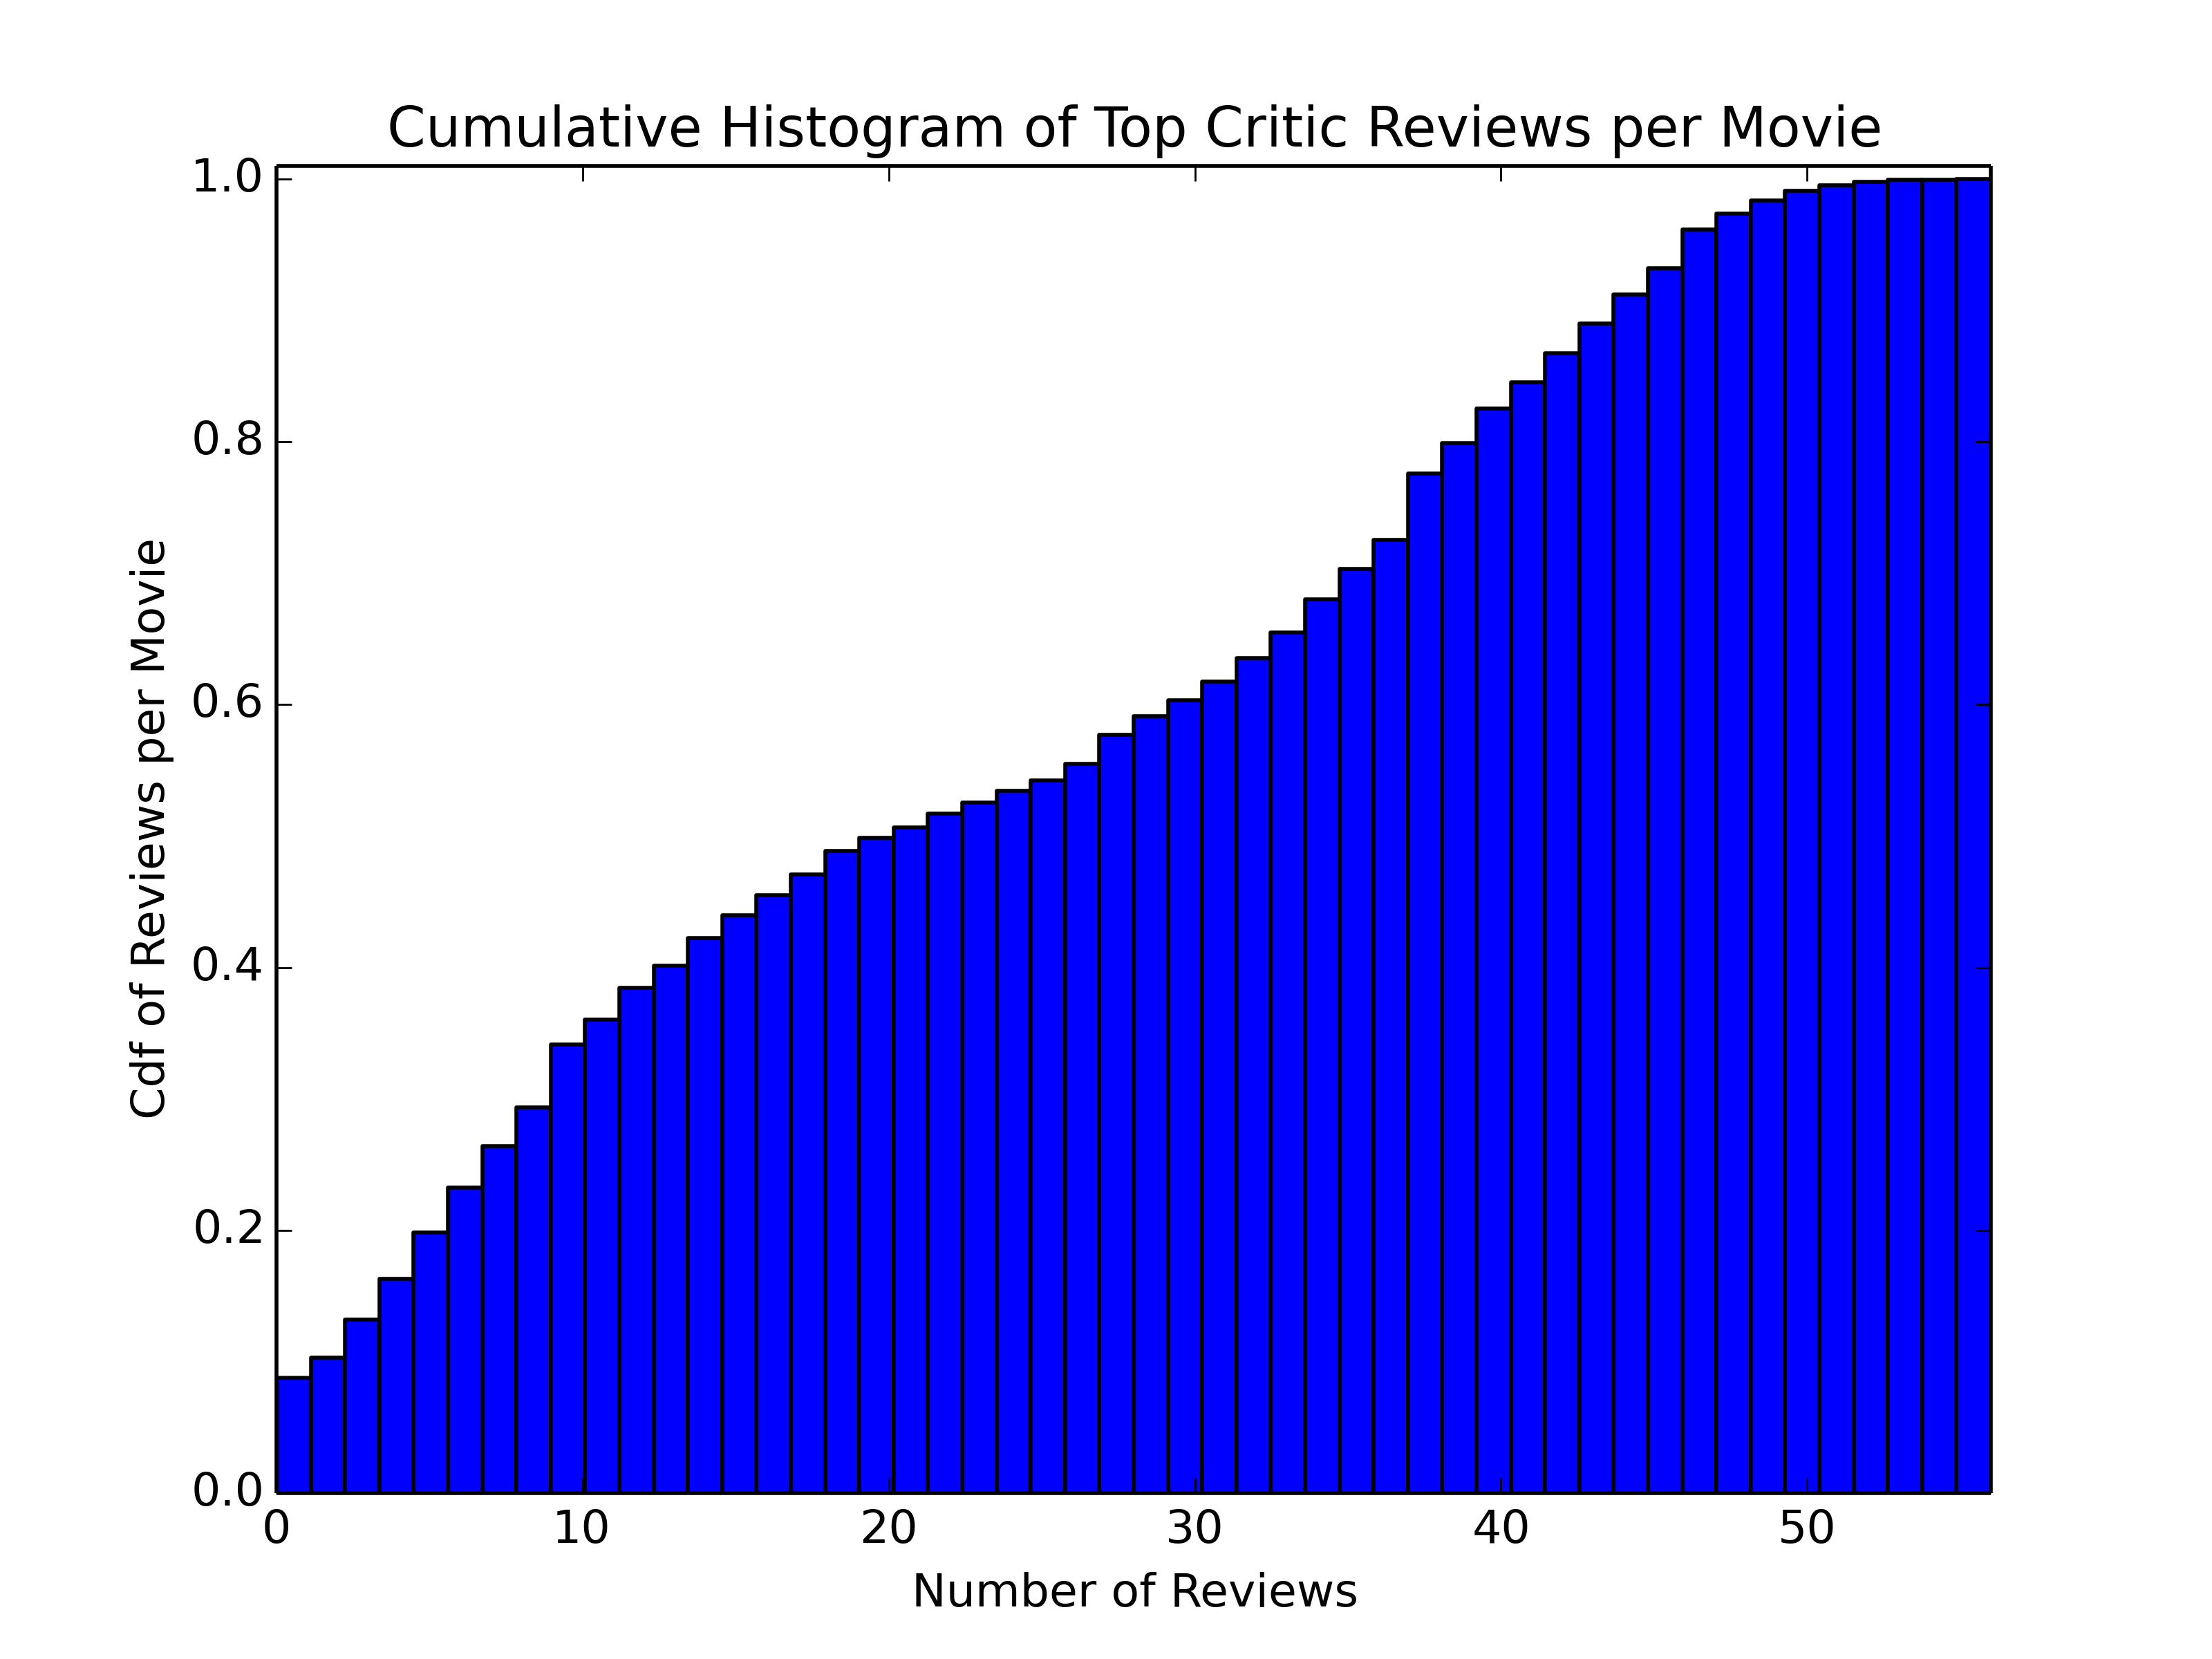
\includegraphics[width=0.48\textwidth]{data_plots/plot_r_mov_top.png}
	    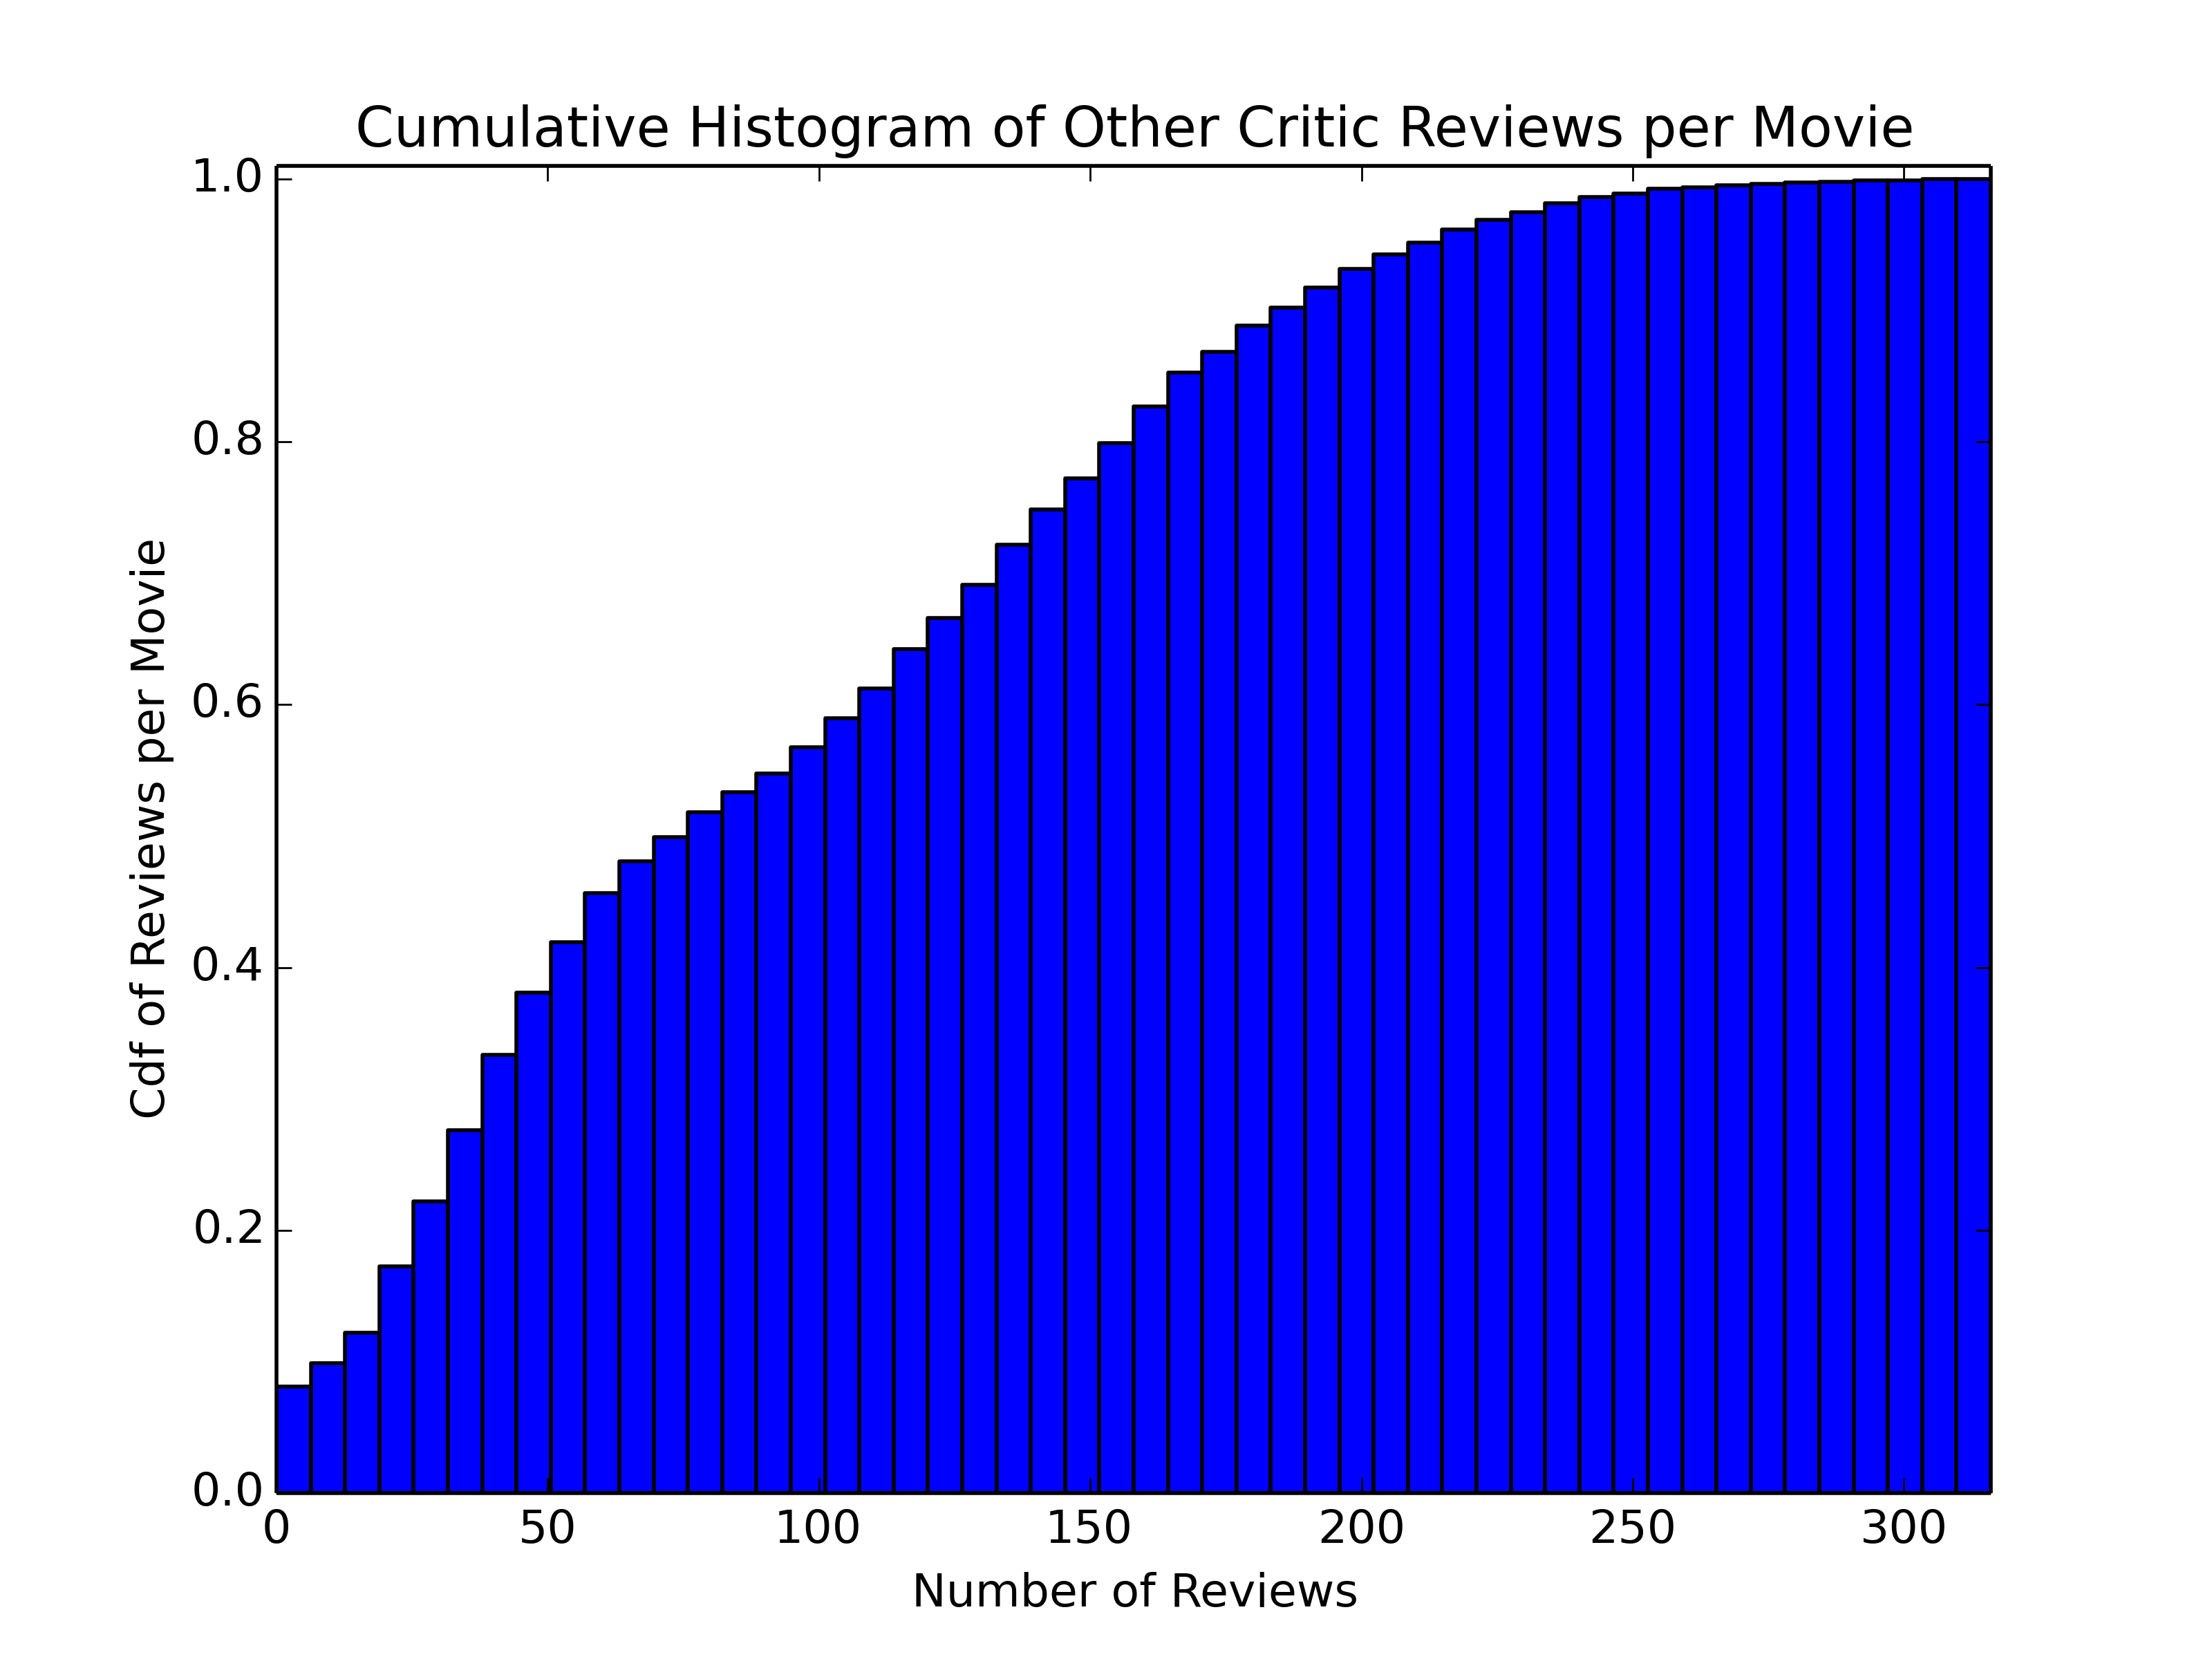
\includegraphics[width=0.48\textwidth]{data_plots/plot_r_mov_oth.png}
	    \caption{Cumulative histograms of critic reviews per movie for movies on Rotten Tomatoes}
	    \label{fig:r_mov} 
	\end{figure}


	\begin{table}[H]
	 \centering
	 \caption{Distribution of number of reviewed movies per critic on rotten tomatoes} 
	 \begin{tabular}{ l | c | c | c | c }
	 \hline
	 &  Min & Max & Mean & Std Dev  \\
	 \hline
	 Top Critcs & 0 & 2862 & 21.79 & 124.96 \\
	 Other Critics & 0 & 2634 & 68.16 & 224.77 \\
	 \hline
	 \end{tabular}
	 \end{table}

	\begin{figure}[H]
	    \centering
	    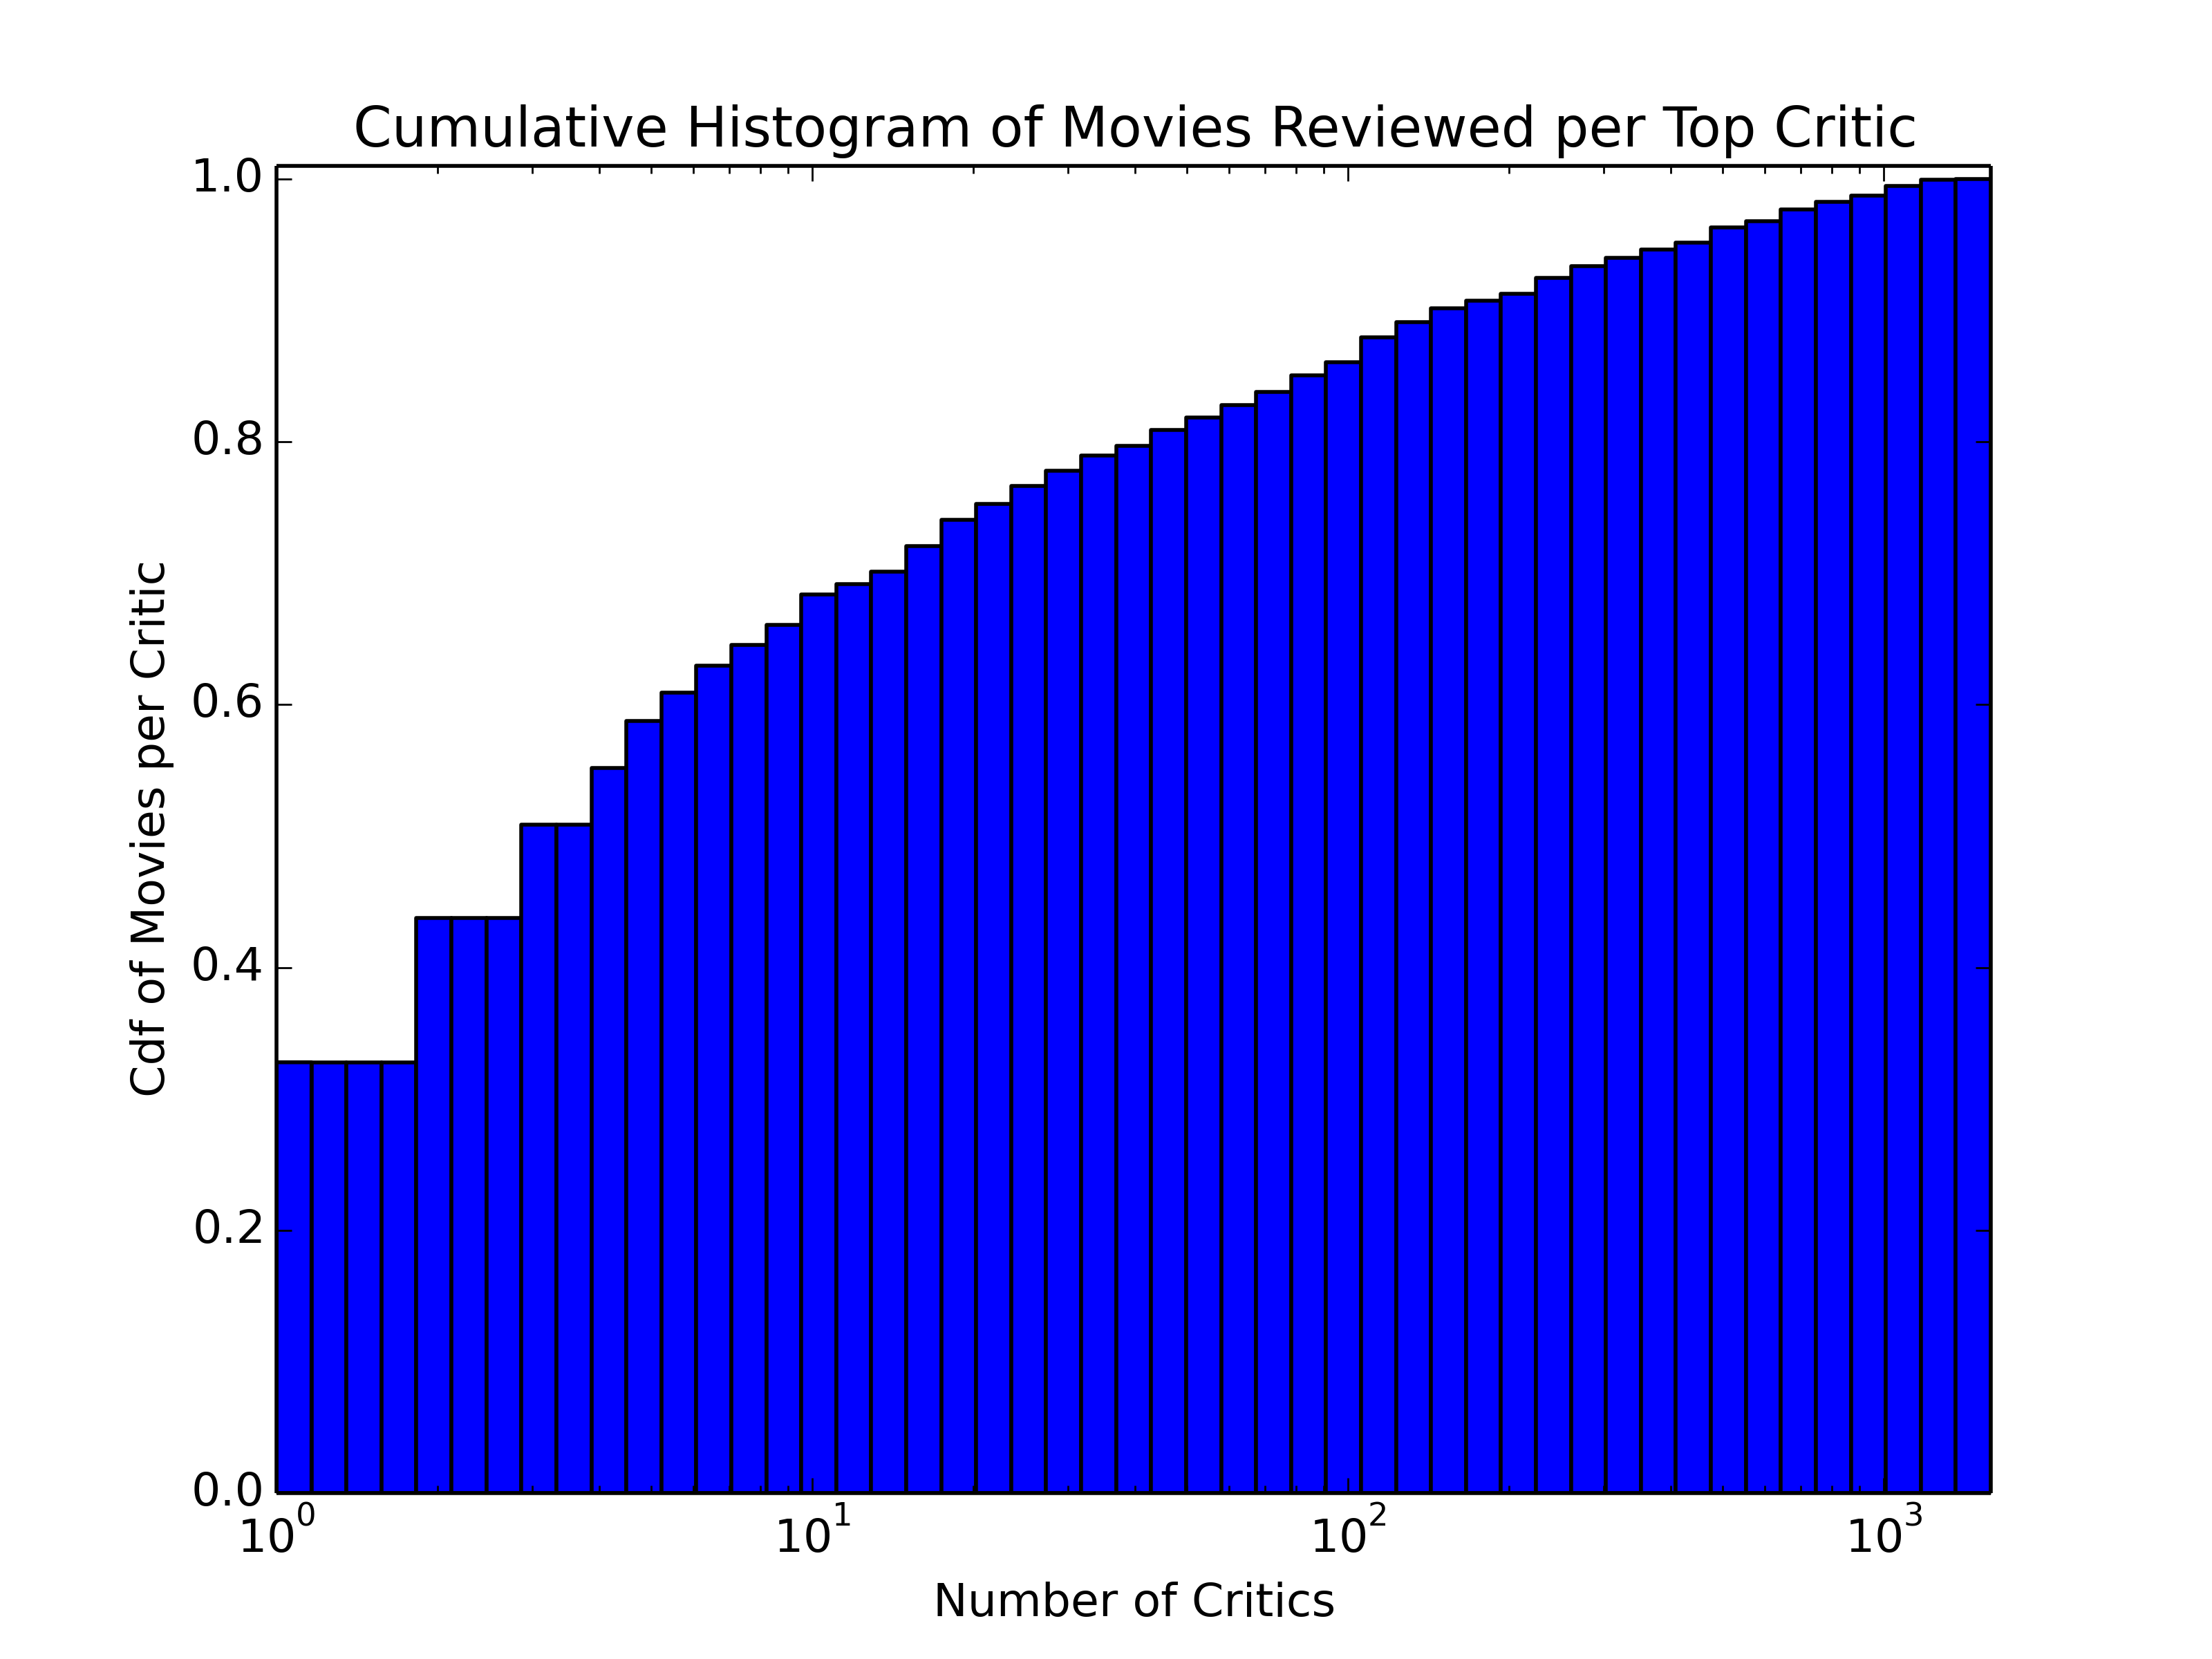
\includegraphics[width=0.48\textwidth]{data_plots/plot_r_crit_top.png}
	    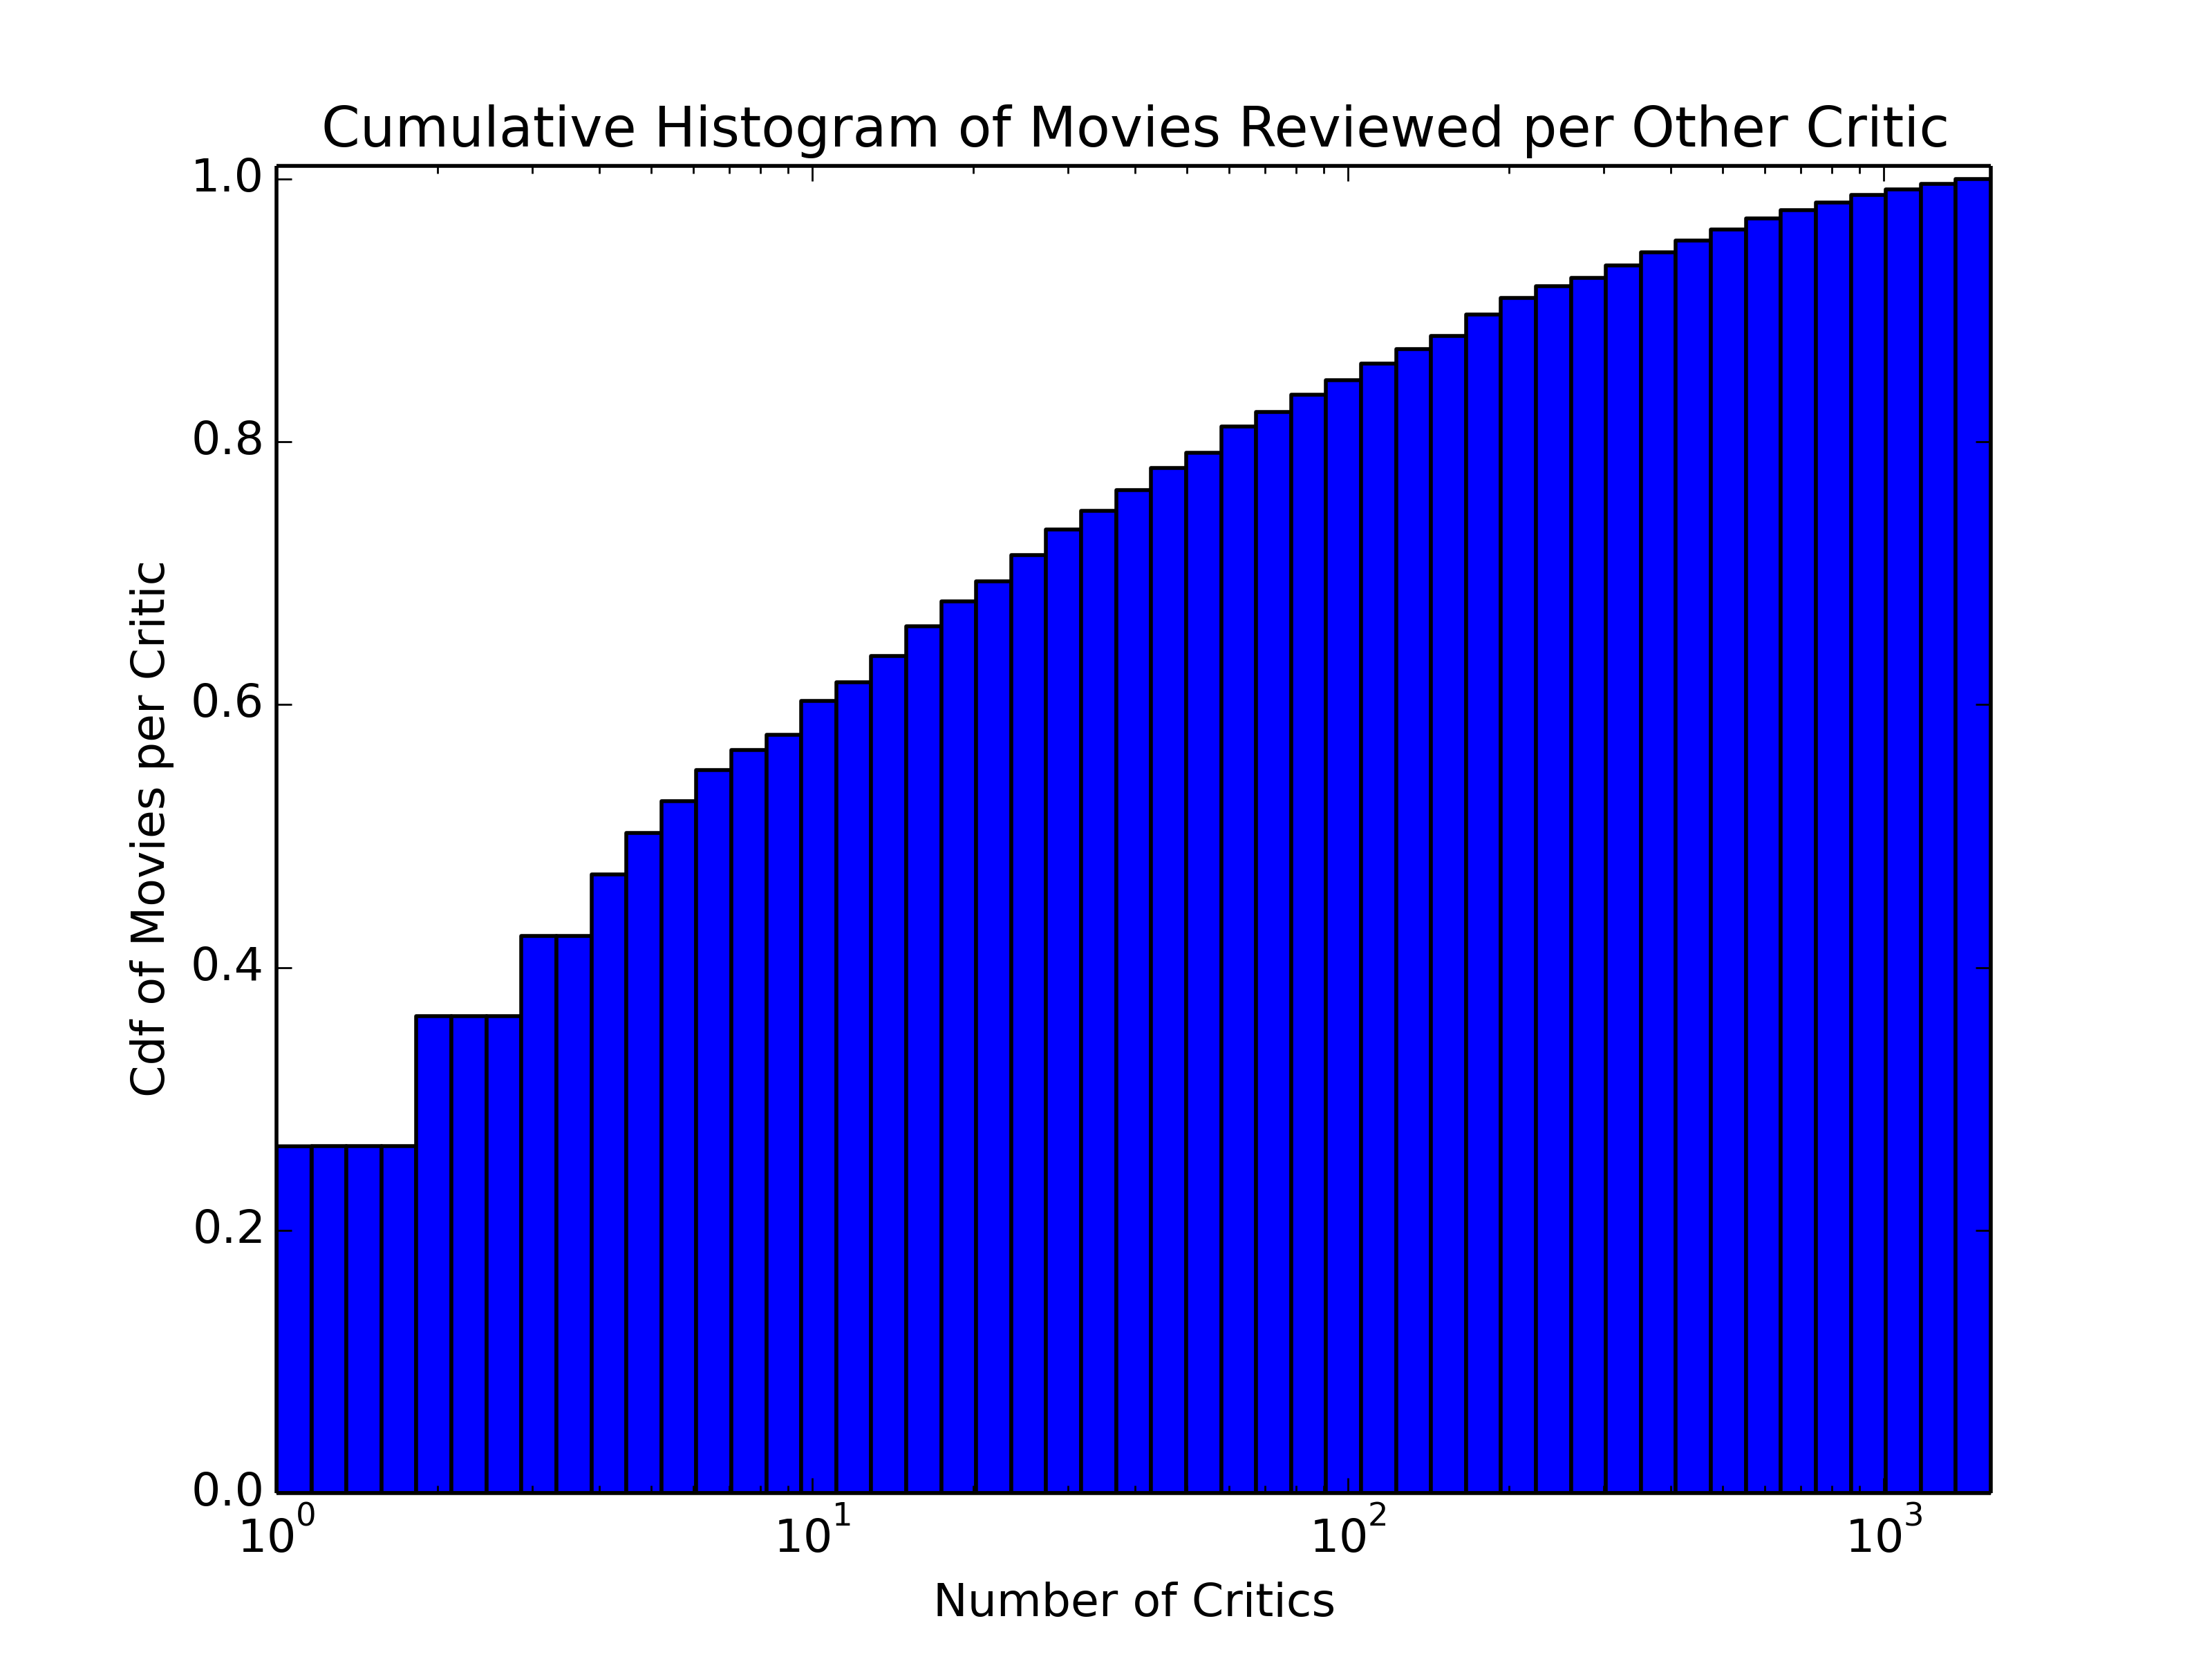
\includegraphics[width=0.48\textwidth]{data_plots/plot_r_crit_oth.png}
	    \caption{Cumulative histograms of the number of movies reviewed by critics on Rotten Tomatoes}
	    \label{fig:r_crit}
	\end{figure}



\section{Matrix factorization results}

Figures 6-9 show some of the results we obtained with this technique. We first tried with only one dimension per user and critic $D=1$. As shown in Figure \ref{fig:1}, this produces quite unimpressive results. This model is far too simple to learn anything particularly interesting. All we can really learn here is how lenient critics are, and the average rating given to a movie.

As we increase the number of features, we see that our training and test error both improve. However, as this occurs the training and test error become less correlated. We see that with a larger number of dimensions we become more vulnerable to over fitting, and the regularization parameter $\lambda$ becomes increasingly important. It is interesting that, throughout our different models, though the training error varies significantly, the test error consistently reaches a minimum at around $0.43$. 

The best test error seems to occur in the most complex model with the highest regularization constant $D=40$, $\lambda = 10$, but it is not much better than the test error achieved in other models.

Since the data has mean zero and standard deviation one, the zero predictor, which assigns a rating of zero to every element would give us an average squared error of $1.0$, and the random predictor who assigns a rating with mean zero and standard deviation would give an average squared error of $2.0$. Our model at $0.43$ does do significantly better than random. However, by incorporating more features into our model we hope to do much better.

	\begin{figure}[H]
	\centering
	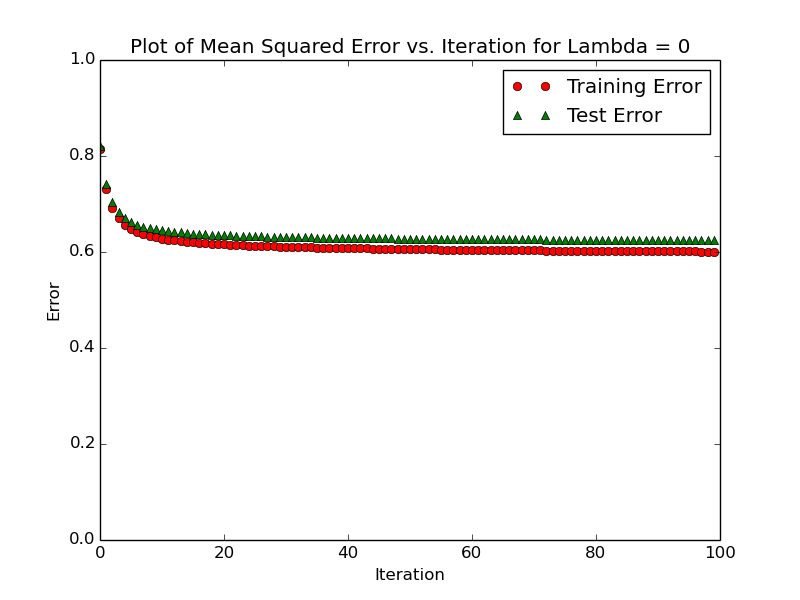
\includegraphics[width=\plotwidth\textwidth]{matrix_plots/test-i100d1l0.png}
	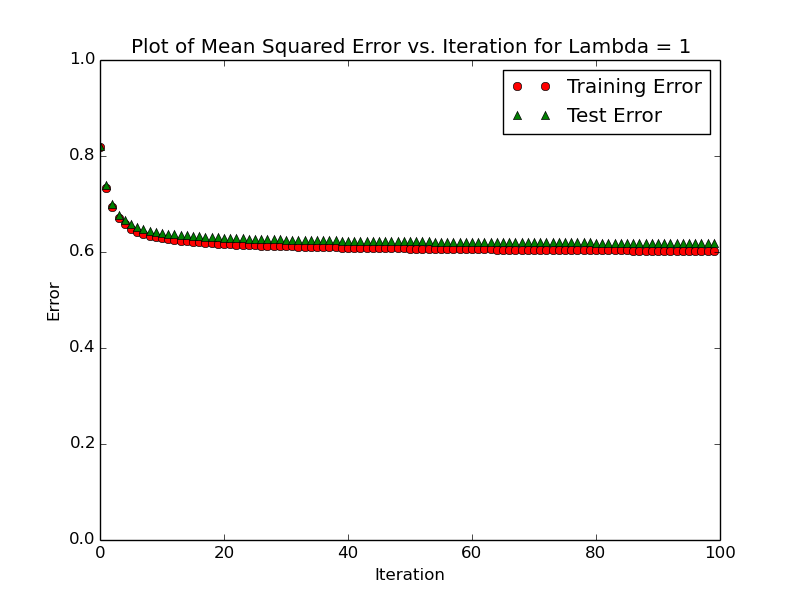
\includegraphics[width=\plotwidth\textwidth]{matrix_plots/test-i100d1l1.png}
	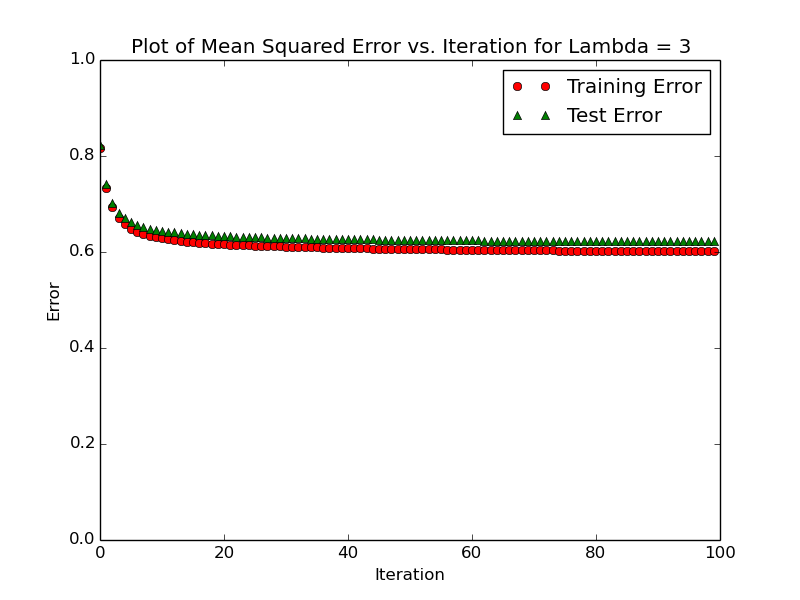
\includegraphics[width=\plotwidth\textwidth]{matrix_plots/test-i100d1l3.png}
	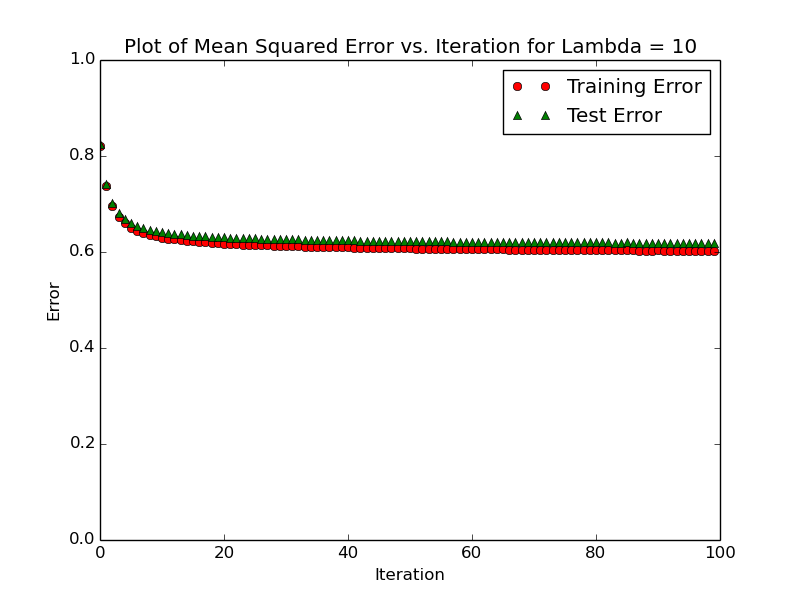
\includegraphics[width=\plotwidth\textwidth]{matrix_plots/test-i100d1l10.png}
	\caption{Mean squared training and test error over 100 iterations in the stochastic matrix factorization model. Stochastic gradient descent was done using a step size of 0.02. The learned critic matrix was count(critics) by 1, and the learned movie matrix was 1 by count(movies).}
	\label{fig:1}
	\end{figure}


	\begin{figure}[H]
	\centering
	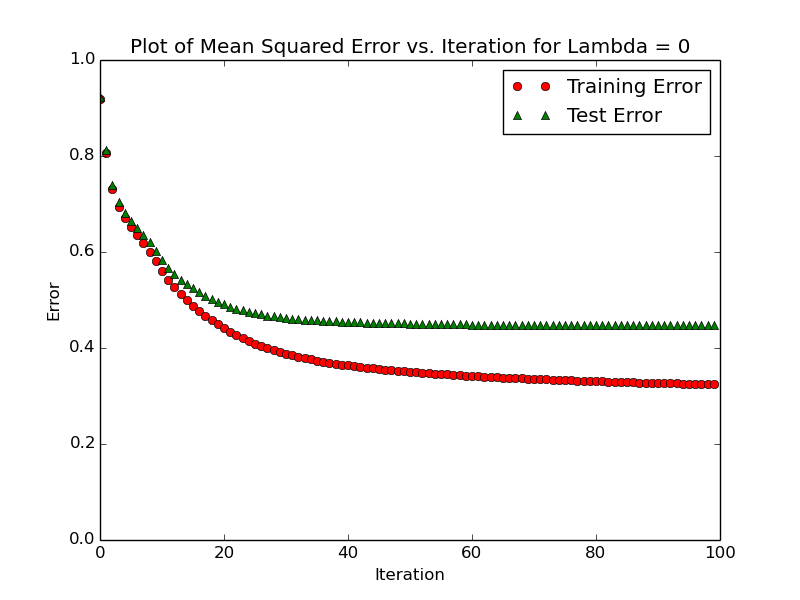
\includegraphics[width=\plotwidth\textwidth]{matrix_plots/test-i100d10l0.png}
	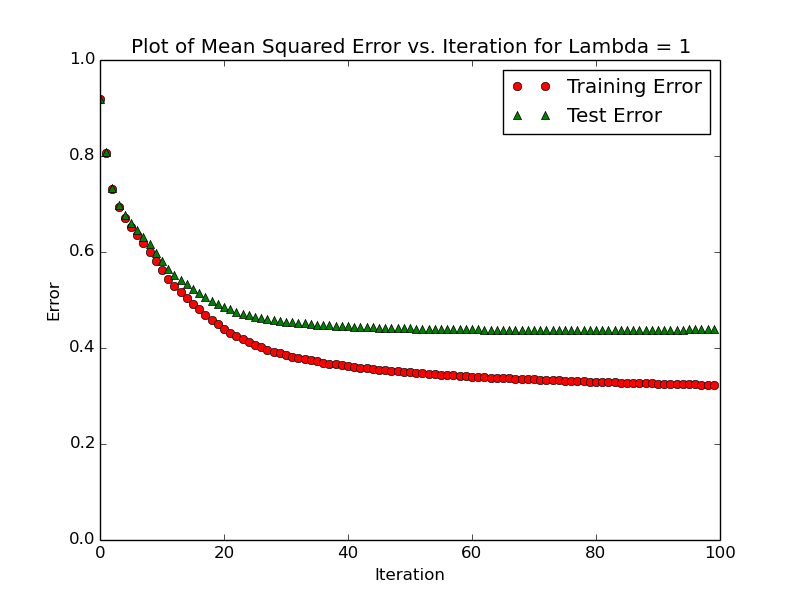
\includegraphics[width=\plotwidth\textwidth]{matrix_plots/test-i100d10l1.png}
	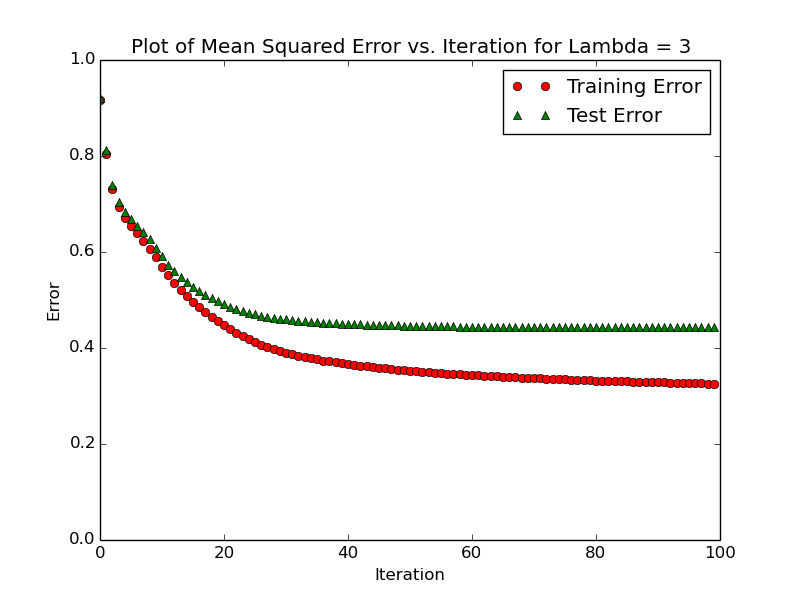
\includegraphics[width=\plotwidth\textwidth]{matrix_plots/test-i100d10l3.png}
	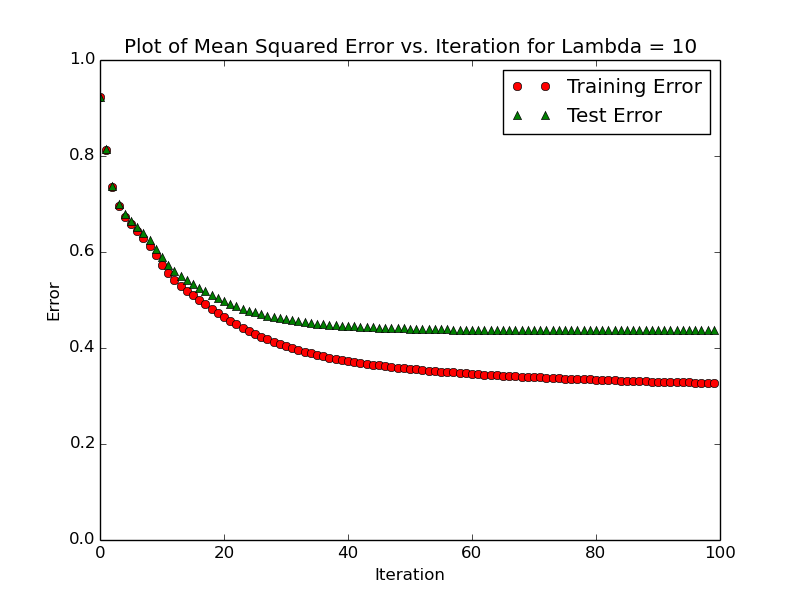
\includegraphics[width=\plotwidth\textwidth]{matrix_plots/test-i100d10l10.png}
	\caption{Mean squared training and test error over 100 iterations in the stochastic matrix factorization model. Stochastic gradient descent was done using a step size of 0.02. The learned critic matrix was count(critics) by 10, and the learned movie matrix was 10 by count(movies).}
	\label{fig:10}
	\end{figure}


	\begin{figure}[H]
	\centering
	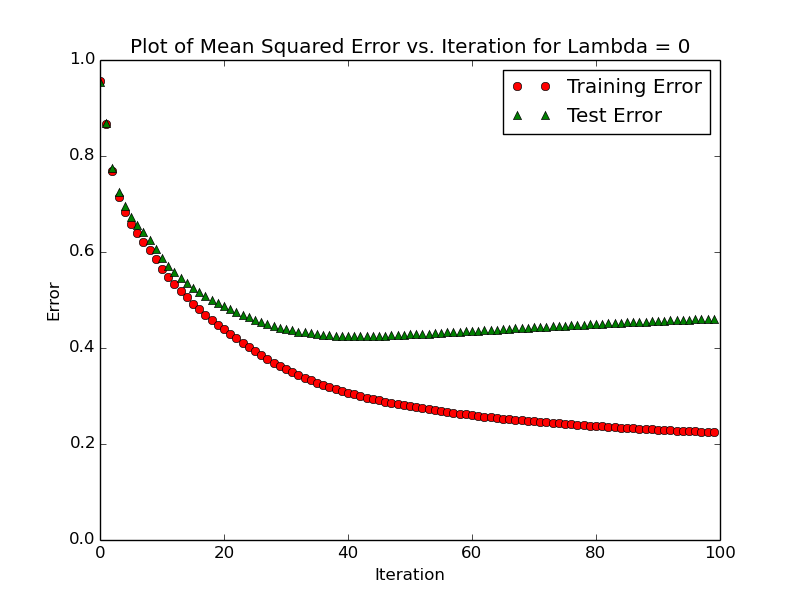
\includegraphics[width=\plotwidth\textwidth]{matrix_plots/test-i100d25l0.png}
	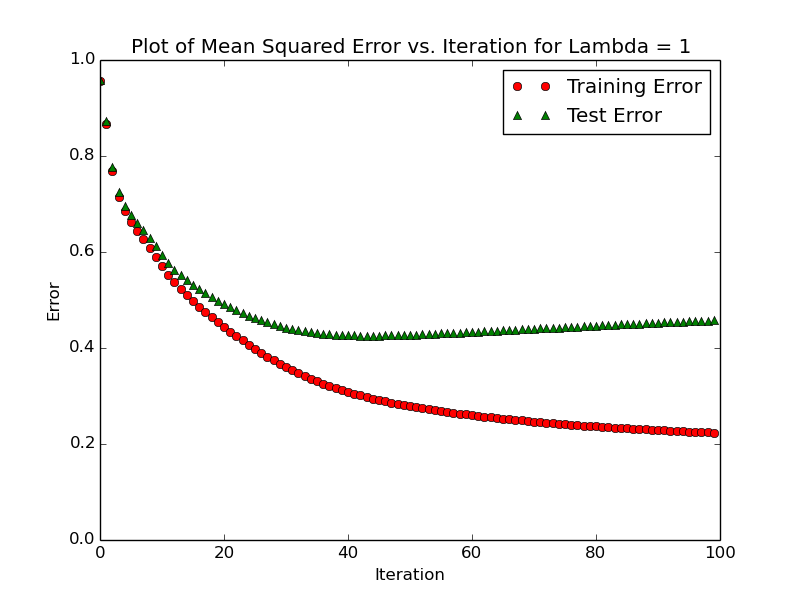
\includegraphics[width=\plotwidth\textwidth]{matrix_plots/test-i100d25l1.png}
	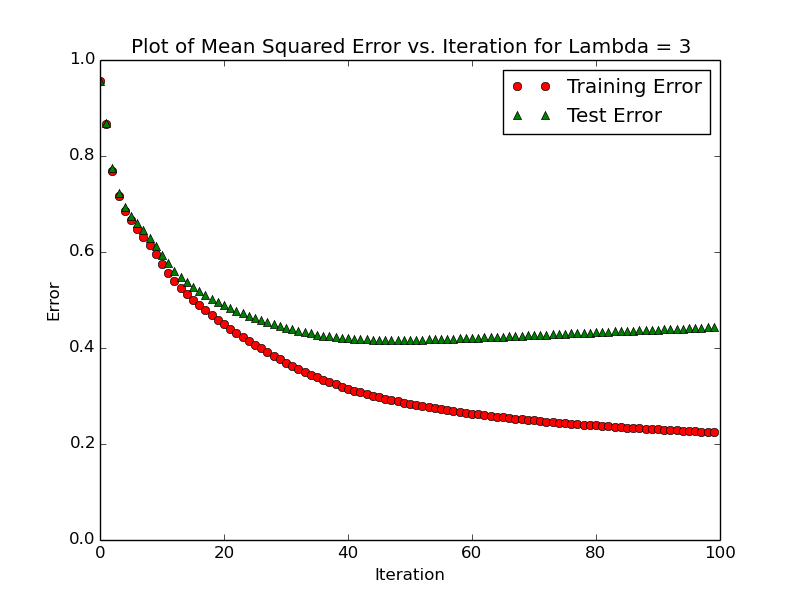
\includegraphics[width=\plotwidth\textwidth]{matrix_plots/test-i100d25l3.png}
	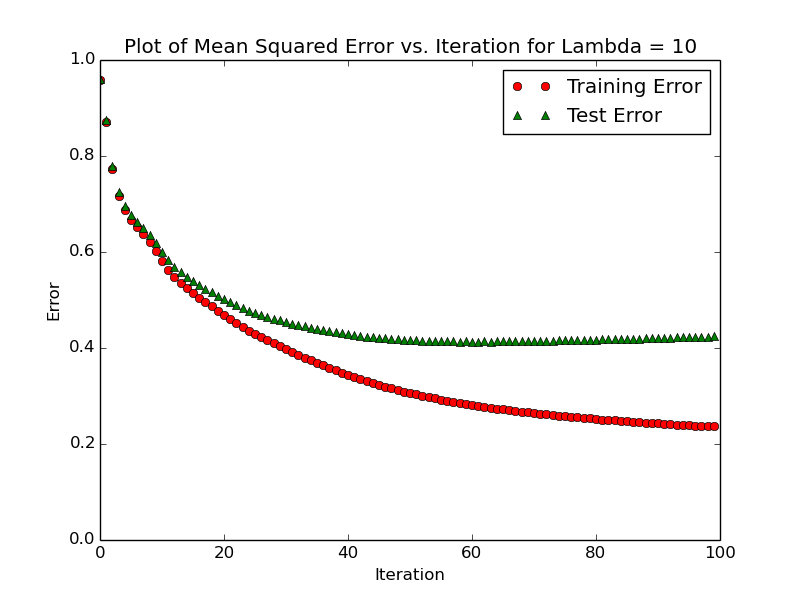
\includegraphics[width=\plotwidth\textwidth]{matrix_plots/test-i100d25l10.png}
	\caption{Mean squared training and test error over 100 iterations in the stochastic matrix factorization model. Stochastic gradient descent was done using a step size of 0.02. The learned critic matrix was count(critics) by 25, and the learned movie matrix was 25 by count(movies).}
	\label{fig:25}
	\end{figure}


	\begin{figure}[H]
	\centering
	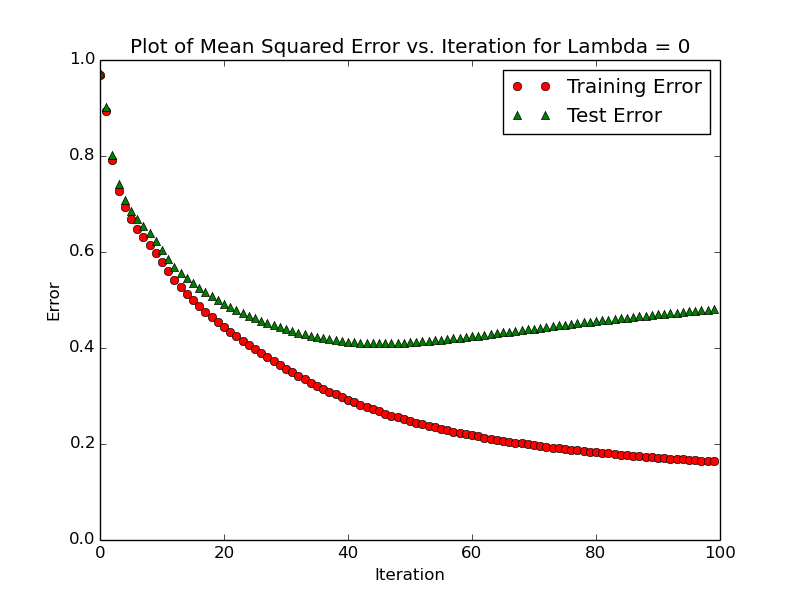
\includegraphics[width=\plotwidth\textwidth]{matrix_plots/test-i100d40l0.png}
	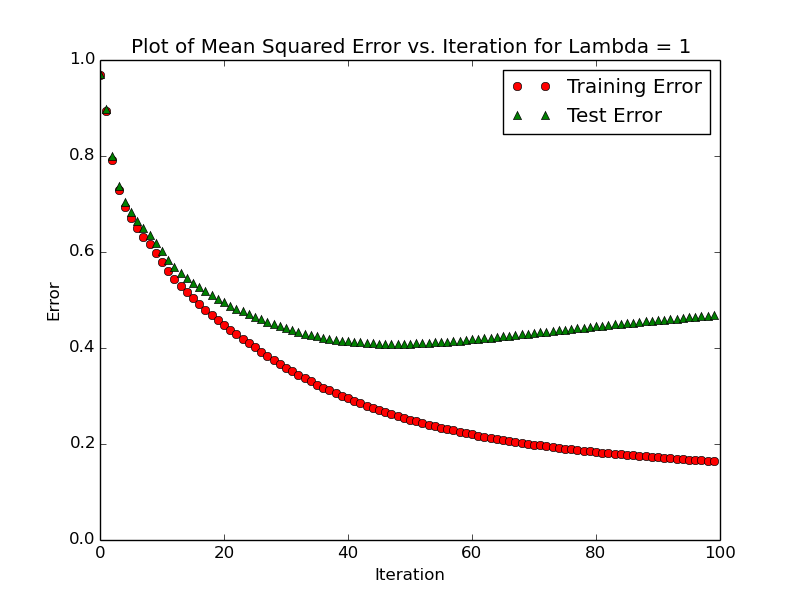
\includegraphics[width=\plotwidth\textwidth]{matrix_plots/test-i100d40l1.png}
	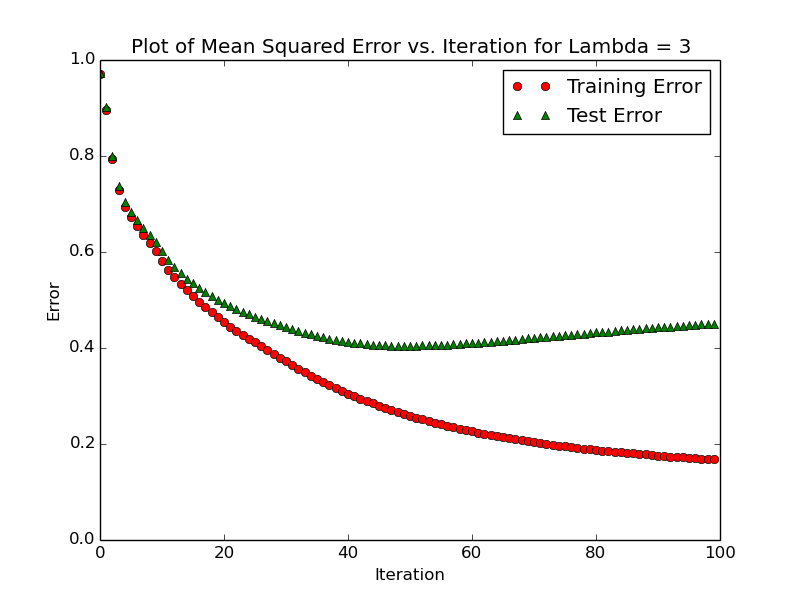
\includegraphics[width=\plotwidth\textwidth]{matrix_plots/test-i100d40l3.png}
	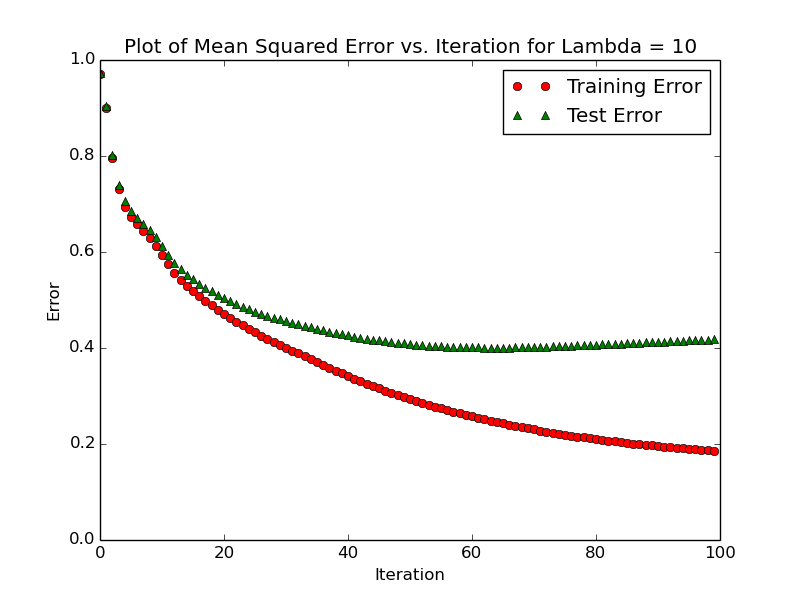
\includegraphics[width=\plotwidth\textwidth]{matrix_plots/test-i100d40l10.png}
	\caption{Mean squared training and test error over 100 iterations in the stochastic matrix factorization model. Stochastic gradient descent was done using a step size of 0.02. The learned critic matrix was count(critics) by 40, and the learned movie matrix was 40 by count(movies).}
	\label{fig:40}
	\end{figure}

\section{Collaborative Filtering Results}


Collaborative filtering results

Predicting critic ratings using collaborative filtering worked quite well. It confirmed that data sparsity can be overcome in the context of movies by relying on the extensive review history of movie critics.

Indeed, using only 10\% of the reviews as training data we were able to reach a 17\% mean error (all movies are rated out of 100).

We furthermore observed that restricting the training data to critics having written a large number of reviews did not have any significant effect on the mean error. Thus the system can be made more performant by ignoring at least half of the reviewers.


\section{Further work}


The second extension would be to extract more features from data we already have (review publication, movie director, cast, runtime, MPAA rating, etc.) and integrate them in our matrix factorization model. Adding these fixed features to the feature matrices would allow us to more accurately learn the remaining features and therefore enable us to learn a better measure of critic similarity.

The third extension would be to do text analysis on reviews in order to extract critic features (vocabulary, length of reviews, \dots) and movie features (we could learn the movie genre, what emotions it evokes, \dots). This would require a significant amount of work, as sentiment analysis is another entire field of machine learning.

\bibliography{bibliography}{}
\bibliographystyle{plain}

\end{document}
